\documentclass{beamer}

%\usetheme{default}
\usetheme{Frankfurt}
\usecolortheme{default}%{seagull}
\usefonttheme[onlylarge]{structurebold}
\setbeamerfont*{frametitle}{size=\normalsize,series=\bfseries}
\setbeamertemplate{navigation symbols}{}

\usepackage[spanish]{babel}
\usepackage[latin1]{inputenc}
\usepackage{times}
\usepackage[T1]{fontenc}
\usepackage{multicol}
\usepackage{tikz}
\usepackage{graphics}
\usepackage{multirow}
\usetikzlibrary{arrows}
\usepackage{multimedia}
\tikzstyle{block}=[draw opacity=0.7,line width=1.4cm]

\newcommand{\redalert}[1]
{
	{\color[rgb]{1,0,0}{#1}}
}

\newcommand{\Titulo}[1]
{
	\begin{center}
		\tikz \draw (0,0) node[fill=green!50,draw]
		{#1};
	\end{center}
}

\title{Graphs with few trivial critical ideals}
\author{Carlos A. Alfaro}
\date{}


\begin{document}

\begin{frame}

	\maketitle

	\vspace{-2cm}

	\begin{center} 
		
\includegraphics[height=1.5cm]{logo-banxico.jpg}
	\end{center}	
\end{frame}


\begin{frame}
	\tableofcontents
\end{frame}


\section{Assumptions}
\subsection*{S}

\begin{frame}
	\begin{columns}[c]
		\column{.5\textwidth}
			\begin{block}{Assumptions on graphs}
				\begin{itemize}
					\item<1> are \alert{connected},
					\item<2> \alert{multiple edges} are allowed, and
					\item<3> \alert{loops} are forbidden. 
					%\item<3> Sumidero
				\end{itemize}
			\end{block}
		\column{.3\textwidth}
			\begin{tabular}{c}
				\visible<1>{
					\begin{tikzpicture}[scale=1]
						\draw (-30:1) node[fill=black!20, draw=black, minimum size=2mm, circle, line width = .3mm] (v1) {\tiny $G_1$};
	    					\draw (90:1)  node[fill=black!20, draw=black, minimum size=2mm, circle, line width = .3mm] (v2) {\tiny $G_2$};
	    					\draw (210:1) node[fill=black!20, draw=black, minimum size=2mm, circle, line width = .3mm] (v3) {\tiny $G_3$};
	    					\draw (-1,1) node (no) {};
	    					\draw (-1,-1) node (so) {};
	    					\draw (1,1) node (ne) {};
	    					\draw (1,-1) node (se) {};
	    					\draw (no) edge[red,line width=.1cm] (se);
	    					\draw (so) edge[red,line width=.1cm] (ne);
		    			\end{tikzpicture}
				} \\
				\visible<2-3>{
					 \begin{tikzpicture}[scale=1]
						\tikzstyle{every node}=[fill=black!20, draw=black, minimum size=2mm, circle, line width = .3mm]
						\path (-30:1) node (v1) {};
	    					\path (90:1)  node (v2) {};
	    					\path (210:1) node (v3) {};
		    				\draw[line width = .3mm] (v1) -- (v2) -- (v3);
		    				\draw (v1) edge[bend left, green, line width = .3mm] (v3);
		    				\draw (v1) edge[bend right,green, line width = .3mm] (v3);
		    				\draw[red, dashed, line width = .3mm] (v2) .. controls (2,1.5) and (2,0.5) .. (v2);
		    	\end{tikzpicture} 
	    			} \\
			\end{tabular}
	\end{columns}
\end{frame}


\section{Critical group}


\subsection*{Laplacian matrix}


\begin{frame}
	
	\frametitle{Laplacian Matrix}
	
	\begin{block}{Definition}
		Let $G=(V,E)$ be a graph, the \alert{Laplacian matrix} $L(G)$ of $G$ is the matrix with rows and columns indexed by the vertices of $G$ given by
	\[
	L(G)_{u v}=
	\begin{cases}
	\deg_G(u) & \text{ if } u=v,\\
	-m_{u v} & \text{ otherwise},
	\end{cases}
	\]
	where \alert{$\deg_G(u)$} denote the degree of $u$, and \alert{$m_{u v}$} denote the number of edges from $u$ to $v$.
	\end{block}
	
\end{frame}


\begin{frame}

	\begin{block}{Definition}
		By considering $L(G)$ as a linear operator on $\mathbb Z^n$, the \alert{critical group} $K(G)$ of $G$ is the torsion part of the cokernel of $L(G)$.
		\[
			coker(L(G))= \mathbb{Z}^{n}/{\sf Im}L(G) = \mathbb{Z}\oplus \alert{K(G)}.
		\]
	\end{block}

\end{frame}


\subsection{Invariant factors}


\begin{frame}

	\frametitle{Invarian factors}	
	
	\begin{block}{Theorem}
		\[
			K(G) \cong \mathbb{Z}_{\alert{f_1}} \oplus \mathbb{Z}_{\alert{f_2}} \oplus \cdots \oplus\mathbb{Z}_{\alert{f_{n-1}}},
		\]
		where \alert{$f_i \leq 0$} and  \alert{$f_i \mid f_j$} for all \alert{$i\leq j$}.
	\end{block}
	
	\pause
	
	The \alert{$f_1, f_2, ..., f_{n-1}$} are called \alert{invariant factors}.
	
	\pause
	
	\begin{block}{Proposition}
		If \alert{$\Delta_i(G)$} is the g.c.d of the $i$-minors of $L(G)$, then \alert{$f_i$} is equal to $\Delta_i(G)/ \Delta_{i-1}(G)$, where $\Delta_0(G)=1$.  
	\end{block}
	
\end{frame}

\subsection{The family $\mathcal G_i$}


\begin{frame}
	\frametitle{The family $\mathcal G_i$}
	
	\begin{block}{Definition}
		Let \alert{$f_1(G)$} be the number of invariant factors of $L(G)$ equal to $1$.
	\end{block}
	
	\pause
		
	\begin{block}{Definition}
		Let $\alert{\mathcal G_i}$ be the family of \alert{simple connected} graphs con $\alert{f_1(G)=i}$.
	\end{block}
	
	\pause
	
	\begin{block}{Example}
		The following graph belongs to $\redalert{\mathcal G_2}$.
		\begin{center}
			\begin{tabular}{c@{\extracolsep{2cm}}c}
				\multirow{4}{2cm}{
					\begin{tikzpicture}[scale=.9]
						\tikzstyle{every node}=[circle, inner sep=0pt, minimum width=5pt] 	
						\draw (-1,1) node (v1) [draw, fill] {};
						\draw (-1,0) node (v2) [draw, fill] {};
						\draw (0,.5) node (v3) [draw, fill] {};
						\draw (1,1) node (v4) [draw, fill] {};
						\draw (1,0) node (v5) [draw, fill] {};
						\draw (-1.3,1.3) node () {\tiny $v_1$};
						\draw (-1.3,-.3) node () {\tiny $v_2$};
						\draw (0,0.2) node () {\tiny $s$};
						\draw (1.3,1.3) node () {\tiny $v_3$};
						\draw (1.3,-.3) node () {\tiny $v_4$};
						\draw (v1) -- (v2) -- (v3) -- (v4) -- (v5) -- (v3) -- (v1);
					\end{tikzpicture}
				}
				& \\
				&
				$
				{\small
					L(G,s)\sim
					\left[
					\begin{array}{cccc}
						       1      &        0         &           0        &        0        \\
						       0      &        1         &           0        &        0        \\   
						       0      &        0         &           3        &        0        \\
						       0      &        0         &           0        &        3         \\ 
					\end{array}
					\right]
				}
				$\\
				&\\
			\end{tabular}
		\end{center}
	\end{block} 
	
\end{frame}


\begin{frame}
	\begin{figure}
		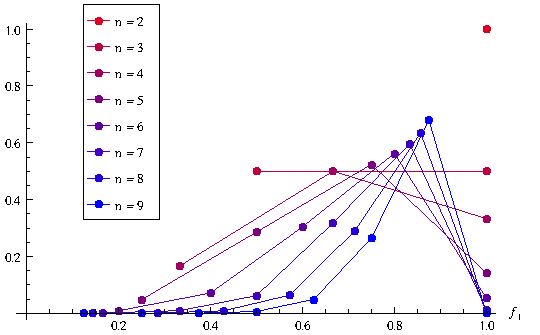
\includegraphics[height=6cm]{InvariantFactors.pdf}
		\caption{N�mero normalizado de graficas con $f_1$ factores invariantes iguales a 1 }
	\end{figure}
\end{frame}


\begin{frame}
	\begin{block}{Pregunta}
		�Qu� tan frecuente es c�clico el grupo cr�tico? es decir, �Qu� tan frecuente $f_1(G)$ es igual a $n-1$ o $n-2$?
	\end{block}
	
	\begin{block}{Conjetura [D. Wagner, 2001]}
		Casi todas las gr�ficas simples y conexas tienen grupo cr�tico ciclico.
	\end{block}
	
	\begin{block}{Teorema [M. Wood, 2014]}
		La probabilidad de que el grupo cr�tico de una gr�fica aleatoria sea c�clica es asint�ticamente a lo m�s 
		\[
			\zeta(3)^{-1}\zeta(5)^{-1}\zeta(7)^{-1}\zeta(9)^{-1}\zeta(11)^{-1} \cdots \approx 0.7935212
		\]
		donde $\zeta$ es la funci�n zeta de Riemann.
	\end{block}
\end{frame}


\begin{frame}	
	
	\frametitle{Gr�ficas con un factor invariante igual a 1}
	
	Por otro lado...
	
	\begin{block}{Pregunta}
		�Qu� podemos decir sobre $\mathcal G_1$?
	\end{block}
%	\begin{block}{Observaci�n}
%		El conjunto $\mathcal G_i$ no es cerrado bajo subgr�ficas inducidas.\\
%		Por ejemplo, el cono de $S_3$ pertenece a $\mathcal G_2$, pero $S_3$ pertenece a $\mathcal G_3$.\\
%		Tambi�n, la gr�fica $K_6\setminus M_2$ pertenece a $\mathcal G_3$, y $K_5\setminus M_2$ pertenece a $\mathcal G_2$.
%	\end{block}
	
	\begin{block}{Teorema [Lorenzini, 1989]}
		Si $G$ es una gr�fica \redalert{simple conexa}, entonces los siguientes enunciados son equivalentes:
		\begin{enumerate}[i.]
			\item $G \in \mathcal{G}_1$,
			\item $G$ es $P_2$-libre,
			\item $G$ es la gr�fica completa.
		\end{enumerate}
	\end{block}
	
\end{frame}


\begin{frame}

	\begin{block}{Pregunta}
		�Qu� podemos decir sobre $\mathcal G_2$ y $\mathcal G_3$?
	\end{block}
	
	\begin{block}{Teorema}
		Sea $G$ una gr�fica \redalert{simple conexa}.
		Entonces, $G\in \mathcal{G}_2$ si y solamente si $G$ es una de las siguientes gr�ficas:
		\begin{enumerate}[i.]
			\item $K_{n_1,n_2,n_3}$, donde $n_1$, $n_2$ y $n_3$ tienen la misma paridad.
			\item $L_{n_1,n_2,n_3}$, si $n_1, n_2, n_3 \geq 3$ tienen la misma paridad, u otros once casos.
			\[
				\begin{tikzpicture}[scale=3]
					\draw[draw=black!40, line width=15pt] (-.5,0) -- (0,0);
					\draw[draw=black!40, line width=15pt] (.5,0) -- (0,0);
					\draw (-.5,0) node[draw, circle, fill=black!40] () {\tiny $K_{n_1}$};
					\draw (0,0) node[draw, circle, fill=white] () {\tiny $T_{n_2}$};
					\draw (.5,0) node[draw, circle, fill=black!40] () {\tiny $K_{n_3}$};
				\end{tikzpicture}
			\]
		\end{enumerate}
	\end{block}
	
	La demostraci�n usa los ideales cr�ticos.
\end{frame}


\begin{frame}

	\begin{tabular}{cc}
		\multirow{7}{5cm}{
			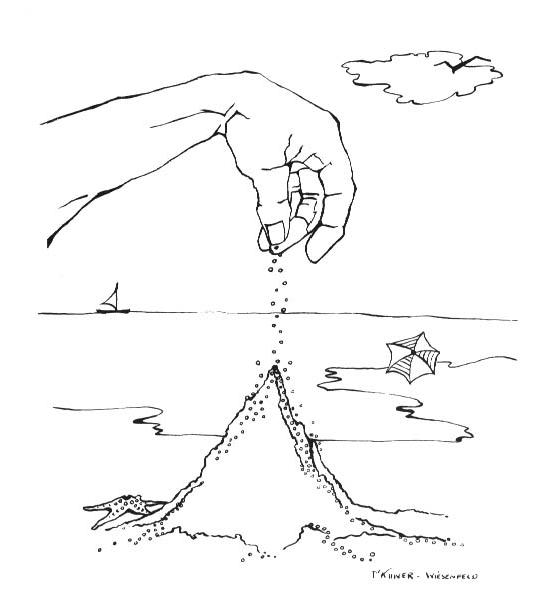
\includegraphics[scale=.25]{mano.jpg}
		}
		& \\

& \\ 		& \\ 
		& �Gracias! \\
		& \\
	\end{tabular}

\end{frame}

\end{document}


